\documentclass[11pt, oneside]{article}   	% use "amsart" instead of "article" for AMSLaTeX format
\usepackage{geometry}                		% See geometry.pdf to learn the layout options. There are lots.
\geometry{letterpaper}                   		% ... or a4paper or a5paper or ... 
%\geometry{landscape}                		% Activate for for rotated page geometry
%\usepackage[parfill]{parskip}    		% Activate to begin paragraphs with an empty line rather than an indent
\usepackage{graphicx}				% Use pdf, png, jpg, or eps� with pdflatex; use eps in DVI mode
								% TeX will automatically convert eps --> pdf in pdflatex		
\usepackage{amssymb}
\usepackage{amsmath}
\usepackage{parskip}

\title{Mean Value Theorem}
%\author{The Author}
%\section{}
% \subsection*{R code}
\date{}							% Activate to display a given date or no date

\graphicspath{{/Users/telliott_admin/Dropbox/Tex/png/}}

\begin{document}
\maketitle
\Large
%\noindent

A man passes a police car at point $A$ doing 60 mph (the speed limit) and 4 minutes later passes another police car at point $B$, also doing 60 mph, yet the second officer writes him a ticket for speeding, justified by the mean value theorem.  The reason:  point $A$ and point $B$ are 5 miles apart, hence the average speed over this interval was 75 mph, and \emph{must at least have been equaled at some point}.

If $f$ is a "nice" function on the interval $(a,b)$ then there exists at least one point $c$ in that interval where

\[ f'(c) = \frac{f(b) - f(a)}{b-a} \]

\begin{center} 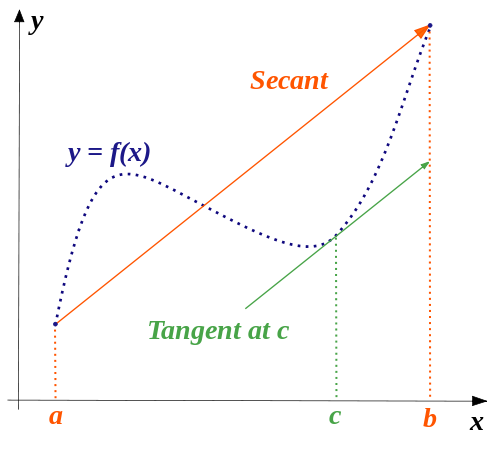
\includegraphics [scale=0.4] {mvt.png} \end{center}

What does it take to be "nice"?  The function $f$ must be continuous over the closed interval $[a,b]$ and differentiable over the open interval $(a,b)$.

The proof of the MVT relies on Rolle's Theorem, which is similar.  Rolle's Theorem says that for a "nice" $f$, if $f(a) = f(b)$, then there will exist at least one point $c$ in the interval $(a,b)$ such that $f'(c) = 0$.  The MVT proof basically turns Rolle's interval so that $a \ne b$.

Problems:




\end{document}  